\documentclass[a4paper,11pt, oneside]{article}  % document class
\usepackage{geometry}
\geometry{
	inner=20mm,
	outer=18mm,
	top=25mm,
	bottom=25mm %
	%  heightrounded,
	%  marginparwidth=50pt,
	%  marginparsep=17pt,
	%  headsep=20pt
}
\usepackage[english]{babel}
\usepackage{hyperref}
%pacchetto
\usepackage{import, multicol,lipsum}  % package
\setlength{\columnsep}{1cm}

\usepackage[utf8]{inputenc} % accenti facili
\usepackage[T1]{fontenc}
\usepackage{subcaption}
\usepackage{pifont}
\usepackage{url}
\hypersetup{
	colorlinks=true,
	linkcolor=blue,
	filecolor=magenta,      
	urlcolor=blue
}
\usepackage{graphicx, color, blindtext}
\usepackage{textcomp, makeidx, times}
\usepackage{amsthm, amsmath, amssymb, amsfonts, mathtools} % math
\usepackage[mathscr]{eucal}		
\usepackage[nottoc]{tocbibind} 
\usepackage{pgfplots, parskip}
\usepackage{afterpage, ifthen}
\usepackage{enumitem}
\pgfplotsset{compat=newest}
\usepackage{graphicx} % immagini
\usepackage{wrapfig}
%\graphicspath{ {image/} } % path cartella delle immagini
\usepackage{tikz} %graph
\usetikzlibrary{arrows,automata}
\usetikzlibrary{automata,arrows,positioning,calc,matrix}
\usepackage[linesnumbered,ruled,vlined]{algorithm2e}
\usepackage{booktabs}
\usepackage{colortbl}
\usepackage{siunitx}
\usepackage{tabularx, tabu}
\usepackage{relsize}
\usepackage{makecell, caption, chngcntr}
\usepackage{bbm}
\usepackage{diffcoeff}
\RequirePackage{fix-cm}


%
%____________________________________________________________________________________________________________________________
%____________________________________________________________________________________________________________________________
%____________________________________________________________________________________________________________________________
%____________________________________________________________________________________________________________________________
% INIZIO
\begin{document}
	
	\setcounter{secnumdepth}{2}
	\pagestyle{plain} % stile pagina (header, numerazioni)
	
	\centerline {
\includegraphics[width=2cm]{logo.jpg}}
	\begin{center}
		Università degli Studi di Torino - M.Sc.  in Stochastic and Data Science - A.Y.  2021/2022 \\
		\Large { Final project of Statistical Machine Learning (MAT0043)}
		\line(1,0){450}\\ 
		\vspace{0.4cm} 
		{ \huge \textbf{Gene selection for cancer type classification} }
		\vspace{0.1cm}
		\line(1,0){450} \\
	\end{center}
	
	%____________________________________________________________________________________________________________________________
	
	The purpose of our project was to work on a high-dimensional genomics data and find a relatively small number of genes to predict the cancer type of a given tumorous cells. This is known as Genes Selection for Cancer Classification and it is in line with many up-to-date problems of applied medicine. \\
	Our dataset contained $1.032$ cancerous cells and their knock-out probabilities, i.e. the probabilities of stopping the growth of tumor by inhibiting one of the $\sim 17.000$ genes. Each cell line was characterized by one of 10 possible cancer labels: Eye, Gastrointestinal, Gynecologic, Musculoskeletal, Neurological, Breast, Head-Neck, Blood, Genitourinary and, finally, Lung. We explored in details three Features Selection algorithms: Random Forests (RF) combined with Feature Importance, Lasso-SVM and Neural Networks (NN) combined with Olden Importance.  We studied two Binary classification problems (Blood cancer vs Rest, Lung cancer vs Rest) and the Multiclass problem. Besides lung models, we achieved satisfying classification accuracies and we were able to select up tp $10\%$ of genes. Models fitted on relevant variables obtained classification accuracies ranging from $67\%$ to $99\%$. \\
	Therefore, it seems that classifying cancer type from an extremely small set of genes depends on the cancer type itself. These methodologies worked incredibly well on Blood cancer, as  we reached almost $100\%$ accuracy with the reduced classifier,  while failed miserably on Lung cancer.  
	
	
	\section{Introduction}
	Cancer is a complex disease characterized by the uncontrolled growth of abnormal cells anywhere in the body. These abnormal cells are extremely invasive and we usually identify them with the name of their original tissue (for instance, breast cancer, lung cancer,  brain cancer, etc.).  In recent years, medicine has made a great step forward in finding new and efficient therapies for different diseases, including cancer.  In particular,  thanks to numerous advances in technology,  collecting huge amount of data is no longer an issue, so that one can exploit information to define personalized treatments for patients. In this regards, the DepMap project\footnote{DepMap Portal: \url{https://depmap.org/portal/} } and,  in particular,  the Achilles project\footnote{Achilles Project: \url{https://depmap.org/portal/achilles/} } aim to use genome-wide screens to collect data regarding mutations of cancerous cells,  identify essential genes and report vulnerabilities across hundreds of human cancers. 
	
	Many researches are currently using DepMap datasets to identify a small number of genes which are responsible of cancers growth\footnote{Background material: \url{https://depmap.org/portal/publications/}}. This procedure is often driven by medical knowledge,  which we do not possess,  together with some rough measures of importance.  Being Maths student, we instead based our research on statistical models and on the hypothesis that "if a given classifier is able to distinguish different types of cancer, then the most relevant genes are the most important features for that classifier" (the meaning of "important" will be clarified later).  Of course,  selecting few truly significant genes has outstanding implications in the medical field: building faster diagnosis tools and synthesizing less toxic drugs are only two examples. 
	
	
	\section{Dataset}
	We used two public datasets from the DepMap Public 21Q3 database,  released on August 2021\footnote{Download dataset from DepMap:  \url{https://depmap.org/portal/download/}}:
	\begin{itemize}
		\item[D1] \textit{CRISPR\_gene\_dependency.csv},  containing $1.032$ cancer cells and their $17.393$ gene scoring results;
		\item[D2] \textit{sample\_info.csv}, containing cell lines information,  such as primary disease and sample collection site.
	\end{itemize}
	Data were collected from real patients and successively processed,  so that element $(i, j)$ of this $(1.032 \times 17.393)$-data frame is the probability that "knocking out gene $j$ has a real depletion effect on the $i$-th cell".
	Before proceeding with our analysis, we removed missing values: only 10 rows coming from different tumours were involved. 
	
	\begin{wrapfigure}{r}{0.65\textwidth}
		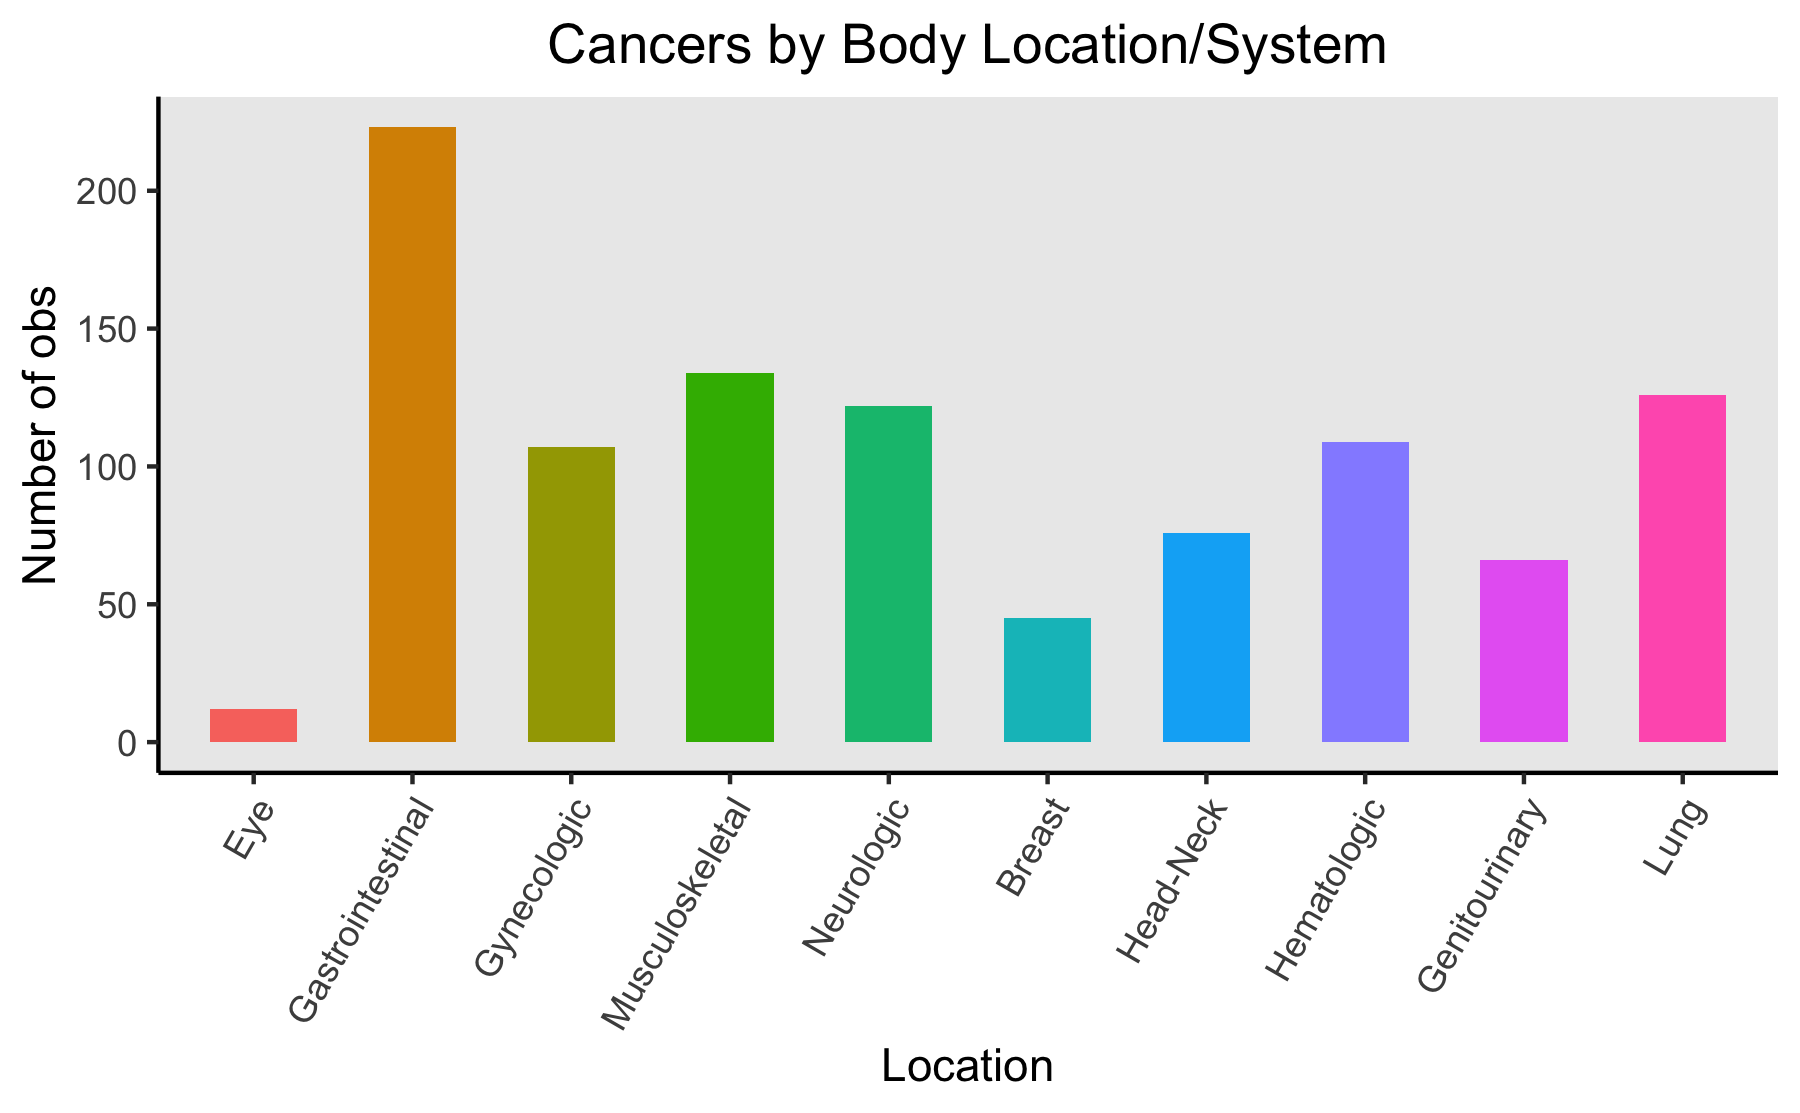
\includegraphics[width=0.55\textwidth]{plot1.png}
		\captionof{figure}{Cancer classes}\label{fig1}
	\end{wrapfigure}
	We grouped the various cancer types in 10 classes according to common medical knowledge\footnote{Cancer types grouped by body location: \url{https://www.cancer.gov/types/by-body-location}} and we obtained classes as reported in Figure \ref{fig1}.  "Eye" was the smallest one as there were only $16$ observations, $5$ of which labelled as "Enginereed". On the other hand, "Gastrointestinal" was the largest group and it comprehended $7$ types of cancer,  making this group quite heterogeneous. \\
	We investigated two Binary classification problems, Blood vs Rest and Lung vs Rest, and the Multiclass problem. We chose "Lung" because of the nature of such a class: it was the most numerous group composed only by Lung cancer samples. The choice of "Blood" was instead driven by some underlying biological knowledge: Blood cancer is quite different from other tumours because
	\begin{itemize}
		\item Leukemia, Lymphom and Myeloma are the main kinds of cancer but they all affect white blood cells;
		\item blood is in the whole body, and so the cancer is, too,	
		%\item not all blood cancers require a treatment, just periodical monitoring.
	\end{itemize} 
	
	\section{Methods}
	Let us briefly illustrate the algorithms we used. Our methodology was characterized by three steps:
	\begin{enumerate}
		\item fit the model using all the features;
		\item identify the most important variables based on some measure of importance;
		\item use these genes to fit a reduced version of the classifier and find out its performance.
	\end{enumerate}
	Clearly, each procedure involved fitting a model twice: the all-features version and the reduced one. We were thus forced to split the dataset into two further chunks. This was crucial to ensure independence of the two models and remove any sort of correlation.
	
	\subsection{Random Forest}
	We started by fitting Random Forest (RF) models as they frequently performs well on imbalanced and correlated high-dimensional data. We used Variable Importance to identify the most relevant features. This measure is calculated in three steps. First, prediction accuracy are measured on the out-of-bag samples. Then, the values of the variable are randomly shuffled, keeping all other variables the same. Finally, the decrease in prediction accuracy on the shuffled data is measured and the mean decrease in accuracy across all trees is reported.  Intuitively, the random shuffling means that, on average, the shuffled variable has no predictive power. \\
Hence, Variable Importance measures how much accuracy decreases because of removing a variable. Here, we used it in two different ways:
	\begin{itemize}
		\item \textit{Cross-validation}: we performed a 5-fold Cross-validation on the model, averaged the importance values and selected the top most important features;
		\item \textit{Boruta algorithm}\footnote{Boruta algorithm: \url{https://www.researchgate.net/publication/220443685_Boruta_-_A_System_for_Feature_Selection}}: Boruta repeatedly measured feature importance and then performed statistical tests to screen out irrelevant features. 
	\end{itemize} 
	
	\subsection{SVM-Lasso}
	Support vector machines (SVM) are based on the idea of finding a hyperplane that best separate classes. Here, we combined this method with the classical Lasso penalty, so that the objective function to be minimized was:
	\begin{equation*}
		\dfrac{1}{n} \sum_{i=1}^n hingeLoss(y_i(x_i w + t)) + \lambda ||w||_1  \qquad	\text{where} \qquad  hingeLoss(z) = max\{0, 1-z\}
	\end{equation*}
	The parameter $\lambda$ has been chosen via cross-validation. Thanks to Lasso penalty, we obtained sparsity in predictors: some $w_i$ were shrunken all the way to zero, whereas the others identified important features. 
	
	\subsection{Neural Networks}
	Neural Networks (NN) are efficient models to capture non-linear relationships between predictors and target variables. In this context, we trained NN with two hidden layers of width $400/500$ and $300$ respectively and we chose \textit{ReLU} as activation function for the hidden layer, \textit{sigmoid} and \textit{softmax} for the output layer of, respectively, binary and multiclass classifications. \\
	Given that the binary problems were a little unbalanced, we tried both the usual \textit{Cross Entropy} loss function and the \textit{Focal Loss}, defined as 
	\begin{equation*}
		FL(z) = \alpha \cdot (1 - z)^{\gamma} \log{z} \text{,  \hspace{3pt} with }z \in [0,1]  \text{ and } \alpha,  \gamma \geq 0
	\end{equation*}
	Note that \textit{Focal Loss} can be extended for dealing with multiclass classification tasks\footnote{Focal Loss: \url{https://arxiv.org/pdf/1708.02002.pdf}}. \\
	Once our NNs were fitted,  we ranked variables according to the Olden Importance measure\footnote{Olden Importance: \url{https://depts.washington.edu/oldenlab/wordpress/wp-content/uploads/2013/03/EcologicalModelling_2004.pdf}}, selected the first ones and trained a reduced version of the classifier on them. We used Olden's importance as it can work with multiple hidden layers and multiclass problems. 
	
	\section{Results}
In the next two subsections we present the results obtained by fitting the models discussed before.  Notice that these results are expressed in terms of average recall,  i.e.  
$\frac{1}{k} \sum\limits_{i = 0 }^k r_i$
where $r_i$ is the rate of correct predictions for class $i$ and where $k$ is the total number of classes.  Otherwise,  if we had used the standard accuracy measure,  which is defined as \textit{total correct prediction / number of observations},  we could have conveyed a misleading message.  For example,  in the Lung vs All classification problem we obtained $90 \%$ accuracy but simply because $10\%$ examples were of class Lung and the classifier always predicted the other class, which is pretty useless.  And indeed,  the average recall is $50 \%$.
	
	\subsection{Binary classifications: Blood vs Rest}
We obtained remarkable results in Blood vs Rest classification.  We initially fit a \textbf{Random Forest} (RF) classifier.  Even though Blood cancer observations were only the $11\%$ of the total,  we did not need any adjustments for the minority class.  Indeed,  thanks to proper tuning on trees parameters and a correction on class weights, we reached $98\%$ of mean accuracy.  For the sake of completeness,  we fit also a RF with Cost-Complexity Pruning and we find the same accuracy.  Then,  we focused on feature selection using both RF Variable Importance and the Boruta algorithm.  As shown in Table \ref{table:selected variables},  Boruta individuated a higher number of important features than our manual method and,  in particular,  they agreed only on $84$ genes.  As mentioned above,  we fit two RFs on a second dataset,  one for each feature selection method.  Besides weighting classes,  no further parameters were specified and,  nevertheless,  both RF classifiers predicted correctly $6$ tumour cells out of $7$,  with an average recall of $92 \%$.
	
As second model,  we explored \textbf{SVM-Lasso} in the way it was described in the previous section.  Being an 
embedded Feature Selection method (i.e.  the learning algorithm intrinsically performs feature selection),  fitting the model already provided 108 important genes,  which are the ones associated with a non-zero weight.  The average recall is now of $97\%$.  Furthermore,  $12$ important features were shared with the RF model,  which made us think that those genes might be of medical importance for real.\\

Furthermore,  \textbf{Neural Network} (NN) classifier achieved outstanding performance as well.  In this case,  instead of tuning the NN's parameters in order to take into account the Blood minority class,  we decided to fit 50 NNs (with the topology described in section 3.3)  on 50 different undersampled dataset and then take the average to make predictions.   Each of these fifty datasets was constructed by retaining all the Blood observations and randomly picking as many Non-Blood observations.  The accuracy we achieved was almost $100\%$,  hence we decided to  select the most important genes according to Olden's importance.  Since NNs are especially suitable in handling high-dimensional data, decided to keep more features than RF and try the simplest NN model,  i.e.  built as a "vanilla" neural net with one single hidden layer.  As a result,  we reached an accuracy of $98.8\%$ for this reduced model,  with all Blood cancer cells classified correctly. 
	
	
	\subsection{Binary classifications: Lung vs Rest}
Unfortunately,  we could not build a proper model for Lung vs Rest.  Even after a tuning of the tree parameters,  the \textbf{RF} was not able to detected the minority class.  Thanks to SMOTE, we adjusted the frequency of those observations from $11\%$ to $50\%$ and the refitted RF gave us a slightly better result: at least one third of Lung cancer cells was correctly predicted.  Similar results were achieved with Minimal Cost-Complexity Pruning.  In any case,  we reported the  average recalls in Table \ref{table:big_models}.  Poorly results were found for \textbf{NNs} as well,  even using the \textit{Focal Loss},  and for \textbf{SVM-Lasso}.  Since all the models were not good enough in classifying Lung cancer, we hypothesized that selecting the most important features was pointless and incorrect in terms of real applications hence no reduced model was fit.
	
	
	
	
	
	
	\begin{table}[h!]
		\caption{Average recall of the models fitted with all the features}
		\centering
		\begin{tabular}{c c c}
			\hline\hline
			Task & RF & NN \\ [0.5ex] % inserts table %heading
			\hline
			Blood & 0.977  & 0.986 \\
			Lung & 0.649  & 0.632 \\
			Multiclass & 0.655 & 0.702 \\ [1ex]
			\hline
		\end{tabular}
		\label{table:big_models}
	\end{table}
	
	\begin{table}[h!]
		\caption{Selected variables}
		\centering
		\begin{tabular}{c c c c c}
			\hline\hline
			Task & RF & Boruta & SVM-Lasso & NN \\ [0.5ex] % inserts table %heading
			\hline
			Blood & 109 & 118 & 108 & 300 \\
			Multiclass & 645 &  41 & --- & 1700 \\ [1ex]
			\hline
		\end{tabular}
		\label{table:selected variables}
	\end{table}
	
	\begin{table}[h!]
		\caption{Average recall of reduced models}
		\centering
		\begin{tabular}{c c c c}
			\hline\hline
			Task & RF & SVM-Lasso & NN \\ [0.5ex] % inserts table %heading
			\hline
			Blood & 0.929 & --- & 0.993 \\
			Multiclass & 0.525 &  --- & 0.494 \\ [1ex]
			\hline
		\end{tabular}
		\label{table:reduced_models}
	\end{table}
	
	
	
	
	
	\subsection{Multiclass classification}
	When working with the multiclass problem we decided to remove the group "Eye" because it was a small heterogeneous group which can be difficult to identify for the classifier (clearly it was pointless to remove it for the two previous tasks as it was contained in the other group).  A part from this,  we still split the dataset into two chunks,  one for finding the important genes and one for fitting and testing the reduced classifiers,  and proceeded in a similar fashion by fitting the same models.
	
	Let us consider the \textbf{RF}  classifier. At first we fitted two of them, the former with balanced weights and the latter balancing the weight by looking at each class ratio. This was done because if we look at the confusion matrix we can see hat most of the missclassification errors are data points classified as Gastrointestinal. Gastrointestinal was the biggest cluster we consider with a lot of different cancers so the genes(i.e. the features) important can be different within the cluster. To limit the weight of Gastrointestinal we decided to tune by hand the class weights. At this point we used cross validation to select five models and we extracted the most important features by looking at their relative importance in every model. We set a threshold to obtain  $465$ features and with this we created a reduced model that we fitted using the validation set we had created at the beginning. At last we used Boruta algorithm to find a different set of important variables and we fitted a RF to compare it with the other reduced model.
	
As before,  \textbf{SVM-Lasso} was the second model we explored.  Although it is a model particularly suited for binary classification tasks, we extended it to the multiclass problem by using the so-called OVO (One vs One) approach,  i.e. we took every possible combination of two classes and,  for each of them,  constructed an SVM-Lasso model.  We then ended up with $ \binom{9}{2} = 36$ models and predictions were determined by seeing which class won more "duels".  Again,  being an embedded model,  feature selection is already achieved by fitting the model once.  The number of genes selected and the average recall are displayed in table CITTTTTT.
	
	Then we moved to \textbf{NNs}.  We fit three different NNs: the first one using the \textit{CrossEntropyLoss},  the second one using the \textit{Focal loss} and the third one using again the \textit{Focal loss},  but changing the $\alpha$ parameter (see section 3.3.) w.r.t.  the class percentages.  The three models held similar results with the second one being slightly more accurate.  We then took it and ranked the variable according to the Olden Importance measure,  selected the first 1700 and used them to construct a reduced version of the classifiers on the second dataset.  The average recall is reported in .  Note that the increment in the number of features used for fitting the reduced model w.r.t. the binary NN model is comprehensible and was due to the fact that separate nine different requires more information. 
	
	
	\section{Conclusion and future works}
As stated in the abstarct,  it seems that classifying cancer type from an extremely small set of genes depends on the cancer type itself.  Our classifiers were able to distinguish Blood cancer almost perfectly but not Lung Cancer,  which can be object of a feature study.  This thesis is supported by the results on the multiclass task were we observed a significant decrease of the average recall due to bad-behaved classes such as Lung (again!) and Gastrointestinal. 
From a more general perspective,  we must also admit that although the selected features are vaguely shared among the three classifiers,  we do not have any hint about which genes they represent and what is their role in the DNA.  In future it could be interesting to involve Med student into a similar project to base our work on a more solid medical knowledge. 
	
	
\end{document}
